% --
% dataset

\section{Dataset}\label{sec:exp_dataset}
This thesis uses two datasets, one is the second version of the speech commands dataset \cite{Warden2018} and the other is self made consisting of only 5 labels (speech commands) that are especially valuable for movement in video games.
The self made dataset is denoted as \enquote{my dataset} and it is merely intended for evaluation.
The training, validation, and testing of the neural network architectures performs on the speech commands dataset.
Both datasets consists of raw waveform files in the \texttt{.wav} format without any feature extraction done beforehand.
As already mentioned in \rsec{prev_kws_benchmark}, the direct comparisons between different neural network approaches is difficult if the feature extraction is left alone to the user.
Some datasets provide feature extraction beforehand, so that the comparability of individual neural network architectures performances is not influenced on it.
The speech commands dataset does not explicitly separate each \texttt{.wav} file into train, test, and validation sets, but provides file lists that refers to distinct waveform files that should be used for testing and validation. 
Hence provides means for comparison to researchers.


% --
% speech commands dataset

\subsection{Speech Commands Dataset}\label{sec:exp_dataset_speech_cmd}
The speech command dataset \cite{Warden2018} consists of \SI{1}{\second} speech recordings, done by over thousands of individual speakers and exists in two versions (\texttt{v0.01} and \texttt{v0.02}).
The first version was published in 2017 with a total number of 30 key words.
In 2018 the second version extended the first version with 5 additional key words \{\enquote{backward}, \enquote{forward}, \enquote{follow}, \enquote{learn}, \enquote{visual}\}.
Further, more class examples were added and a better quality check was conducted in order to remove bad quality recordings.

In this thesis, the experiments are solely performed on the second version \texttt{v0.02} of the dataset with hard-facts listed in \rtab{exp_dataset_hard_facts}.
\begin{table}[ht!]
\begin{center}
\caption{Hard facts of the speech commands dataset \texttt{v0.02}.}
\begin{tabular}{ M{5cm}  M{2cm} }
\toprule
%\textbf{label} & \textbf{train} \\
%\midrule
Total number of key words & 35\\
Total number of examples & 105886\\
Total number of speakers & 2618\\
\midrule
%Number of core key words & 20\\
%Number of auxiliary key words & 15\\
Recording duration & 0.4 - \SI{1}{\second}\\
Channels & Mono\\
Bit depth of audio files & \SI{32}{\bit}\\
Sampling frequency & \SI{16}{\kilo\hertz}\\
\bottomrule
\label{tab:exp_dataset_hard_facts}
\end{tabular}
\end{center}
\end{table}
\FloatBarrier
\noindent


All available speech command key words with their separation in training, test, and validation set are shown in \rtab{exp_dataset_all_labels} located in the appendix.
Some key words have a significantly higher number of examples per class than others.
This inconsistency of examples per classes, emerged from the recording settings as described in \cite{Warden2018}, where the main key words were recorded with a higher number of examples from the same speaker.
For instance the same speaker creates five samples of \enquote{go} and two of \enquote{marvin}.
This makes the key words separable into so called \emph{core key words} and \emph{auxiliary key words}.
The core key words are the main classification objective and each core key word should correspond to one individual class label.
Therefore the core key words have the higher count of samples with about 3700 to 4000 examples each.
In detail the core key words are \{\enquote{yes}, \enquote{no}, \enquote{up}, \enquote{down}, \enquote{left}, \enquote{right}, \enquote{on}, \enquote{off}, \enquote{stop}, \enquote{go}, \enquote{zero}, \enquote{one}, ..., \enquote{nine} \}.

The auxiliary key words have the purpose to disturb the classification of the core key words.
Therefore the auxiliary key words should be labeled separately with one single class label.
In many papers those auxiliary key words are labeled as \enquote{unknown}.
However, in this thesis it is referred as \enquote{\_mixed} label, since it is a mixture of all auxiliary key words and core words that were not used for classification.
The \enquote{\_mixed} key words represent all unknown words that a user might speak and are therefore a very important element in the KWS task for the identification of words that are not in the class dictionary.
Note that the \enquote{\_mixed} label makes the classification task much more challenging because the network has to be more accurate in modeling each core key words against the other core key words, and additionally, to the auxiliary key words.
In the creation of the examples for the \enquote{\_mixed} label, it is preferable to have an equal number of examples per individual auxiliary key word and unused core key words.
This was done by placing all unused core key words and auxiliary words into a separate folder and reading them into an ordered list.
This list is ordered such that one example per key word is placed consecutively to the next and repeated until all examples were added.
The auxiliary key word examples picked for training are referenced by the entries of the ordered list, starting from index 0 to the number of training examples per class.

To examine the recorded examples from the speech command dataset, \rfig{exp_dataset_speech_cmd_wav_grid} shows one example from all available speech commands and presents them in raw audio format, where vertical lines indicate the onset detection and end of a \SI{500}{\milli\second} window.
\begin{figure}[!ht]
  \centering
    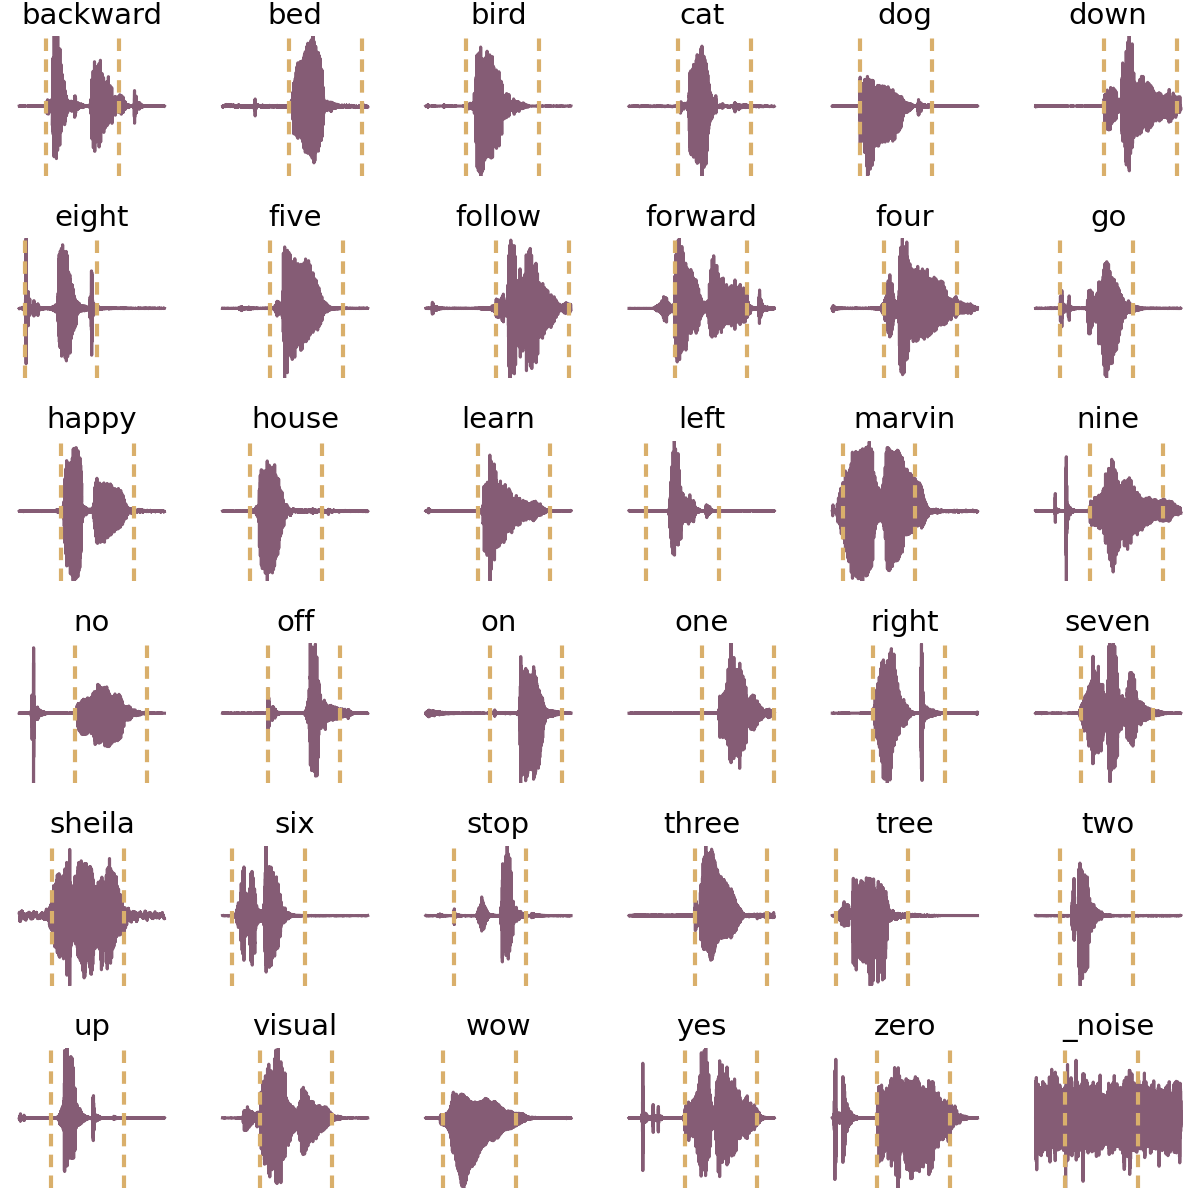
\includegraphics[width=0.65\textwidth]{./5_exp/figs/exp_dataset_speech_cmd_wav_grid.png}
  \caption{One random sample of each individual speech command in the speech command dataset in normalized raw audio format.}
  \label{fig:exp_dataset_speech_cmd_wav_grid}
\end{figure}
\FloatBarrier
\noindent


% --
% statistics

\subsubsection{Observations of all examples in the dataset}
Two histograms were created to observe the quality of all recorded files in the dataset.
Those histograms present an energy measure and a count of the sample length for each file.
The energy of a recorded file provides information about a recordings amplification setting and is an indicator for too silent or too loud (overdrive distortions) samples.
In the first version of the speech command dataset (\texttt{v0.01}) too silent files were a problem.
This had been fixed in the second version by rejecting those silent files, therefore \texttt{v0.01} is slightly more unclean than \texttt{v0.02}.
The energy value $e \in \R$ can be computed as:
\begin{equation}\label{eq:exp_dataset_energy}
  e = \frac{1}{n} \left( \bm{x}^T \bm{x} \right)
\end{equation}
where $\bm{x} \in \R^n$ represents a single recorded file with a total number of $n$ samples.
The division through the sample length $n$ of each individual audio recording is required because not every file has a duration of \SI{1}{\second} (16000 samples).
For an unknown reason many of the recordings consist of less than 16000 samples.
It would be problematic if the sample length is too low to capture a word.
The minimum duration of all examples was found to be about \SI{0.4}{\second}.
This however, is enough for words like \enquote{go} where the reduced samples length often show up.
\rfig{exp_dataset_hist} shows the mentioned histograms of all available examples in the dataset.
\begin{figure}[!ht]
  \centering
    \subfigure[energy measure]{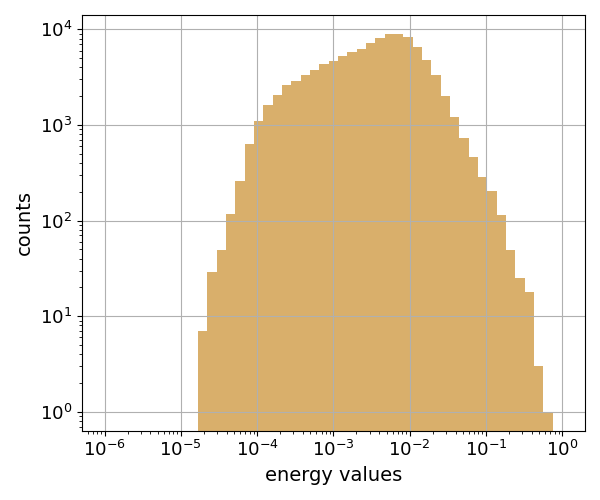
\includegraphics[width=0.42\textwidth]{./5_exp/figs/exp_dataset_hist_energy_overall.png}}
    \qquad
    \subfigure[count of sample length]{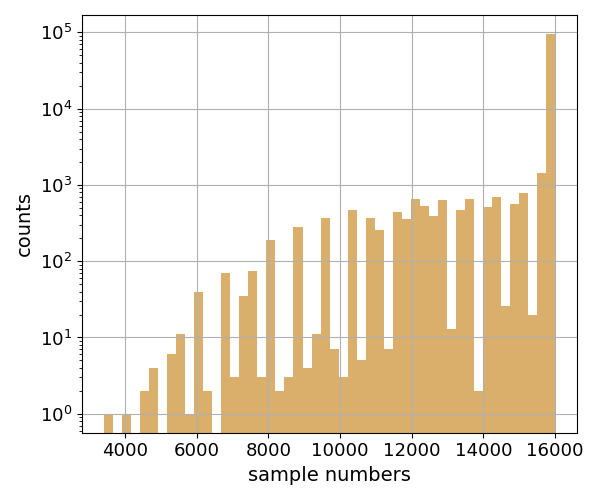
\includegraphics[width=0.42\textwidth]{./5_exp/figs/exp_dataset_hist_sample_overall.png}}
  \caption{Histograms of all examples in the speech commands dataset \texttt{v0.02}, where one histogram shows an energy measure in log-log scale and the other a count of the sample length in log scale.}
  \label{fig:exp_dataset_hist}
\end{figure}
\FloatBarrier
\noindent
The histogram of the energy measure has one main lobe, which is good, so it means that there are no clusters of extremely silent or loud files.
For comparison, if silent files were extracted from for instance the given background files, the energy of some of those would be in a range of $10^{-7} \dots 10^{-6}$.
The sample length histogram shows that most of the files consist of 16000 samples but many others have a smaller number of samples. 
This is important and has to be regarded in the pre-processing of audio files because inputs to neural networks must often be prepared to fixed size inputs if no sequential neural networks, such as RNNs, are used.


% --
% recording quality

\subsubsection{Recording Quality and Personal Experience}
The examples of the speech commands dataset \cite{Warden2018} were not recorded by professionals with high-end recording equipment.
In fact the recordings had been done in an amateur kind of fashion, so that the dataset is more suited to realistic environments intended for user applications.
This is also noted in the paper \cite{Warden2018}:
\begin{quote}
...This meant that the use of studio-captured samples seemed unrealistic, since that audio would lack background noise, would be captured with high-quality microphones, and in a formal setting. 
Successful models would need to cope with noisy environments, poor quality recording equipment, and people talking in a natural, chatty way...
\end{quote}
The recording devices of the speakers, who contributed examples to the dataset, were in most cases simple consumer microphones, as for instance embedded microphones in laptops or mobile phones.

The personal experiments obtained by listened to the examples in the dataset, were as follows:
\begin{itemize}
  \item The quality of the examples in the dataset are ranging from good and understandable to very bad, noisy, unrecognizable and cut off, though most of the examples are provided with good quality.
  \item Different accents had been perceived that suggests that people from several nationalities were involved.
  However, the bias was laid on American English, as noted in the paper.
  \item No children speakers had been found.
\end{itemize}
Due to data privacy issues the information of individual speakers is not displayed.
Therefore, it is not clear whether the dataset consists of an equal amount of male and female speakers and whether there are any children speakers included.
The last would be especially interesting for a video games intended for children.

In many recordings the background noise is imminent, such as traffic noise, chattering people, office sounds, and many more.
A quality check of the recorded files in the dataset had been done beforehand to ensure that bad quality examples are rejected.
Nevertheless, there are still some existing flaws such as extremely loud or silent recordings, examples with inconsistent sample numbers, recordings that include too much noise or in the worst case noise only (very rarely), and cut off signals capturing only half of a word.
Those quality issues in the dataset can for most cases be neglected or fixed, such as inconsistent sample numbers. 
Other more problematic cases, such as noise-only examples, should ideally be removed.
But since their occurrence is very rare it is not worth the effort.
Besides, it is usually not a problem for neural networks to cope with noisy datasets.
In many cases it is favorable when a dataset contains many noisy samples so that neural networks can learn invariance against noise, loudness differences, and other nuisances during training.
Moreover, if the training dataset is large enough, and the test and validation sets do not contain very bad examples, there should be no problem in the training and evaluation of different models.
Finally, it has to be acknowledged that the dataset is published under the creative common license, hence it is freely available to everyone, which is simply fabulous.


% --
% dataset structure

\subsubsection{Dataset Structure}\label{sec:exp_dataset_structure}
The speech command examples are stored in separate folders named after each individual key word.
The folder named as \texttt{\_background\_noise\_} contains six different background noise files, such as \texttt{white\_noise.wav} or \texttt{doing\_the\_dishes.wav}, with a duration of more than one minute each and altogether summing up to a duration of about \SI{400}{s}.
To extract noise examples from those files with a sufficient number of examples of over 3500, those noise files have to be extracted by a striding window of \SI{1}{\second} length shifted by \SI{0.110}{\second}.
The noise examples were assigned to the label \enquote{\_noise}.

Each waveform file from the key word folders is named by an 8-digit hexadecimal hash code for the speaker identification and followed by the utterance number, for instance \texttt{3b4f8f24\_nohash\_0.wav}.
With the speaker identification code known it is possible to distinguish between different speakers.
However, as mentioned above, no further information about the speakers is provided due to data privacy issues.

Moreover, the dataset contains a testing file list called \texttt{testing\_list.txt} and a validation file list \texttt{validation\_list.txt}, where each row entry in the text file refers to a file in the dataset, as for example \texttt{right/bb05582b\_nohash\_3.wav}.
Those file lists should ensure the comparability between different neural network approaches from individual researchers.
The testing and validation file lists are applied in this thesis and the separation into sets are shown in \rtab{exp_dataset_all_labels}.


% --
% extracted examples

\subsubsection{Samples from the Feature Extraction}
The feature extracted data examples are stored to separate files before using them for training.
This has the practicability that features do not have to be extracted each time a new training instance of a neural network is performed.
Samples from the extracted MFCCs with frame-based normalization, as explained in \rsec{signal_mfcc}, are shown in \rfig{exp_dataset_speech_cmd_mfcc}.
\begin{figure}[!ht]
  \centering
    \subfigure[left]{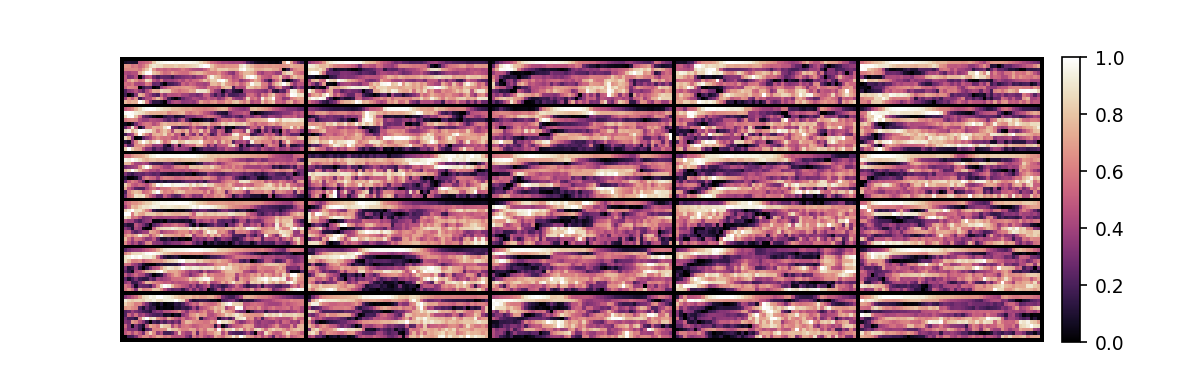
\includegraphics[width=0.45\textwidth]{./5_exp/figs/exp_dataset_speech_cmd_mfcc_left.png}}
    \subfigure[right]{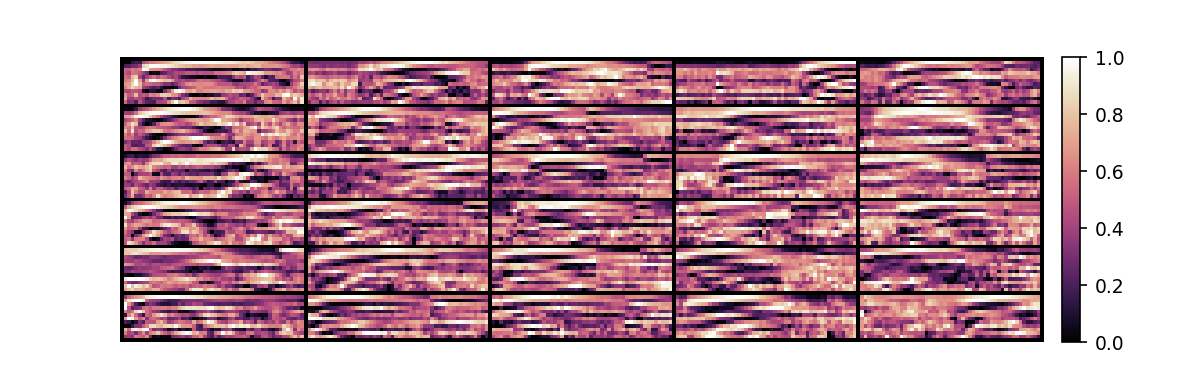
\includegraphics[width=0.45\textwidth]{./5_exp/figs/exp_dataset_speech_cmd_mfcc_right.png}}
    \subfigure[up]{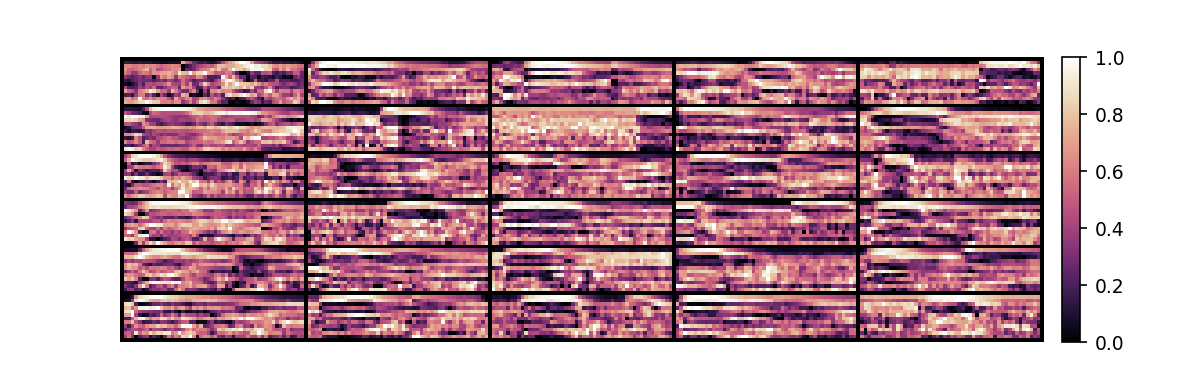
\includegraphics[width=0.45\textwidth]{./5_exp/figs/exp_dataset_speech_cmd_mfcc_up.png}}
    \subfigure[down]{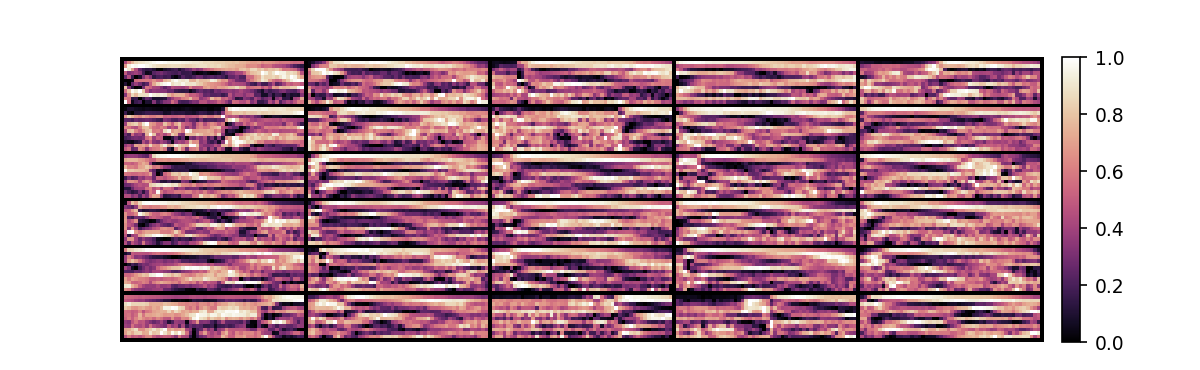
\includegraphics[width=0.45\textwidth]{./5_exp/figs/exp_dataset_speech_cmd_mfcc_down.png}}
    \subfigure[go]{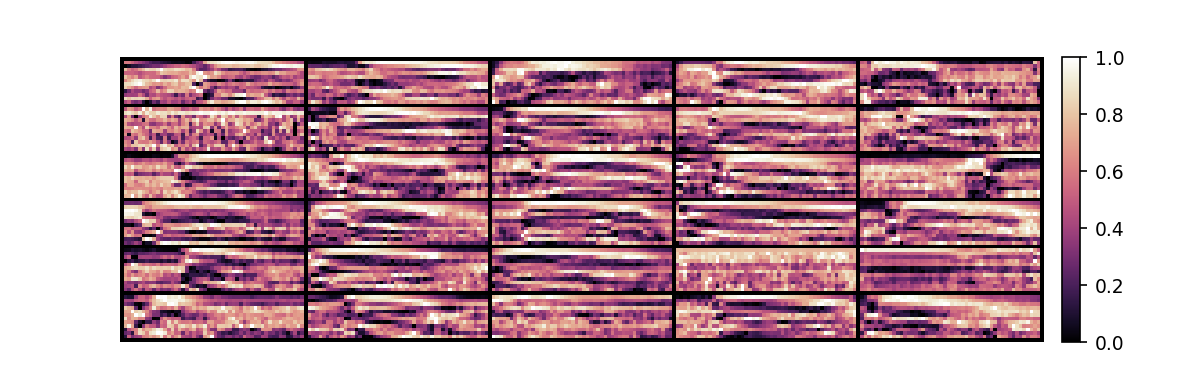
\includegraphics[width=0.45\textwidth]{./5_exp/figs/exp_dataset_speech_cmd_mfcc_go.png}}
  \caption{MFCC extraction of randomly selected 30 samples per class label, obtained from the training set of the speech commands dataset \texttt{v0.02}. The corresponding class labels are written below the plots.}
  \label{fig:exp_dataset_speech_cmd_mfcc}
\end{figure}
\FloatBarrier
\noindent


% --
% my dataset

\subsection{My Dataset}\label{sec:exp_dataset_my}
This dataset was created by the author of this thesis and contains five examples for each of the following key words \{\enquote{left}, \enquote{right}, \enquote{up}, \enquote{down} and \enquote{go}\}.
The datasets purpose is mainly to have an additional test set for evaluating trained models on the authors own voice.
The examples per key word are spoken with different emphasis and stress on individual phonemes for each key word.
Also the prolongation of the words are different, for instance that in one example the word is spoken very hasty and in the other it is spoken slowly.
The emphasis and prolongation ensure the diversity of the dataset.
It is important to mention that none of the self recorded files were used within the training set, so that the neural networks performance is evaluated on unseen data.
All examples of \enquote{my dataset} are illustrated in \rfig{exp_dataset_my_wav_grid} in raw audio format.
\begin{figure}[!ht]
  \centering
    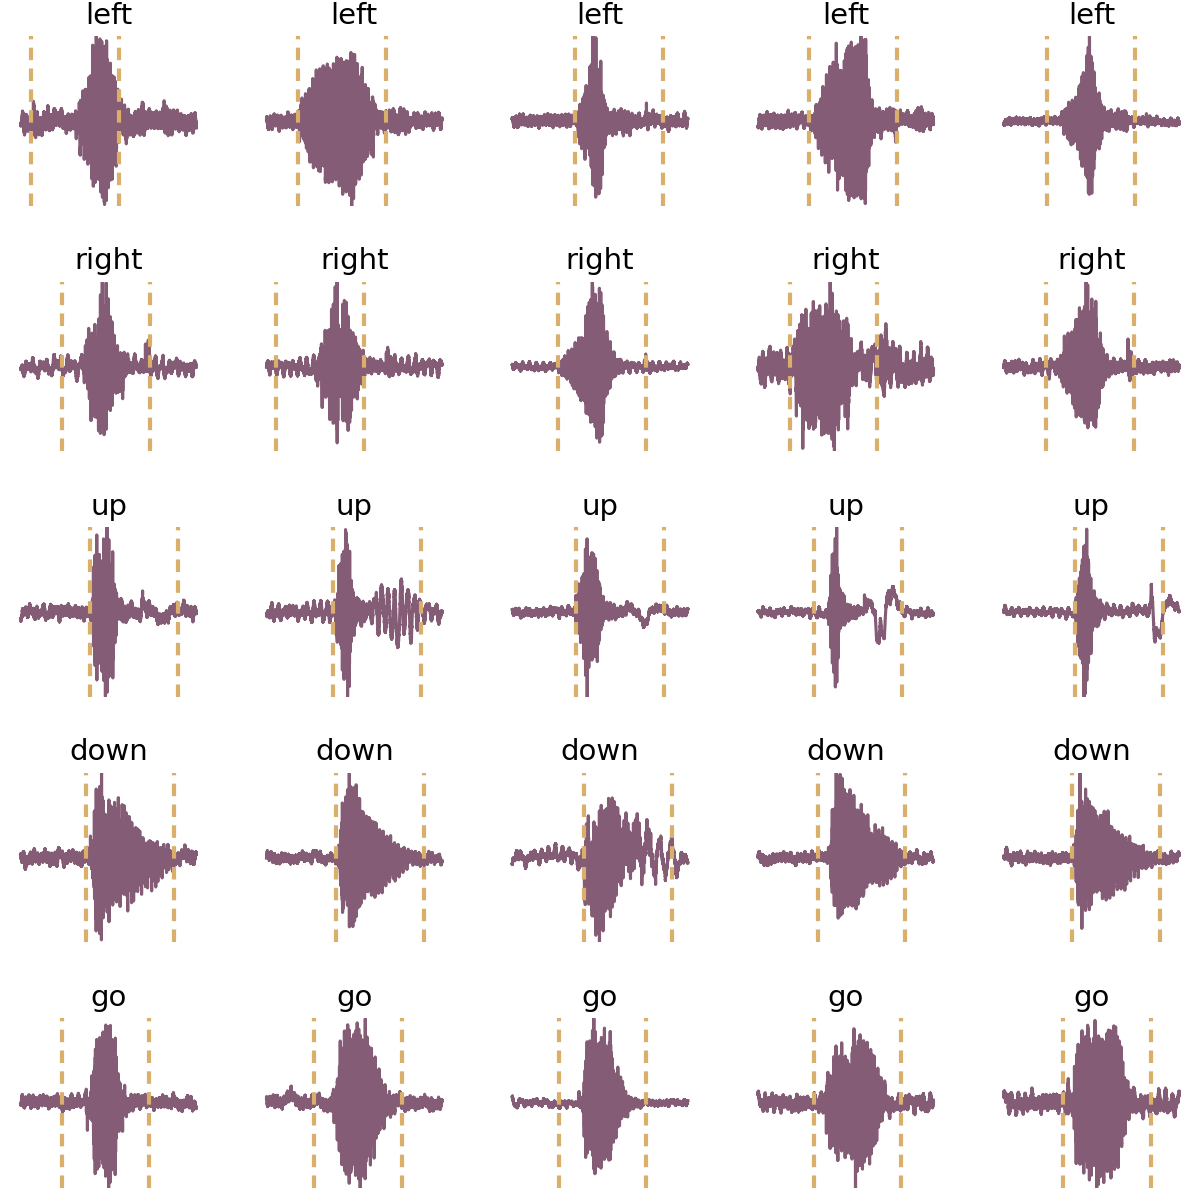
\includegraphics[width=0.6\textwidth]{./5_exp/figs/exp_dataset_my_wav_grid.png}
  \caption{Self recorded files of the \enquote{my dataset} in raw audio format.}
  \label{fig:exp_dataset_my_wav_grid}
\end{figure}
\FloatBarrier
\noindent
The same examples extracted to MFCC features are shown in \rfig{exp_dataset_my_mfcc}.
\begin{figure}[!ht]
  \centering
    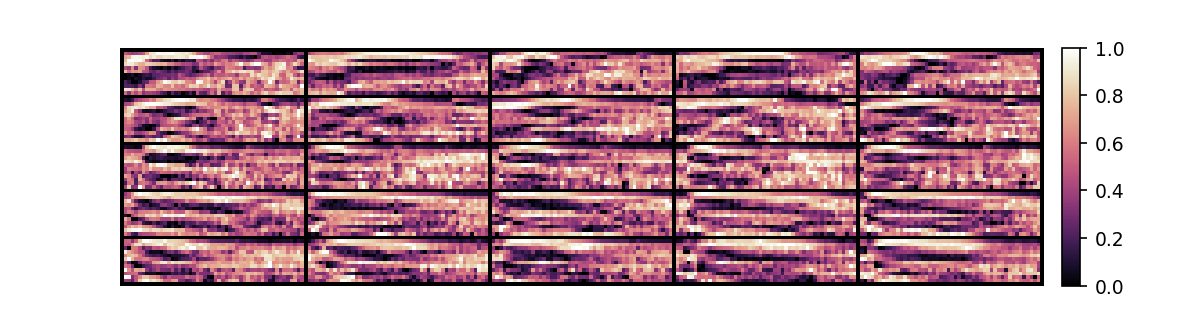
\includegraphics[width=0.65\textwidth]{./5_exp/figs/exp_dataset_my_mfcc.png}
  \caption{All MFCC extracted samples of the \enquote{my dataset} with the same ordering as shown in \rfig{exp_dataset_my_wav_grid}.}
  \label{fig:exp_dataset_my_mfcc}
\end{figure}
\FloatBarrier
\noindent
It turned out that it is a very hard task for neural networks to achieve a \SI{100}{\percent} classification score upon it, despite the fact that all examples correspond to the same speaker.
This is slightly worrying because acoustically each of the examples per word is perfectly understandable for humans and for instance in the classification of the five examples of \enquote{left} from the \enquote{my dataset}, neural networks may classify 4 examples as \enquote{left} and one as \enquote{right}.
It is difficult to examine why exactly this single example is wrongly classified.


% --
% preparation for neural networks

\subsection{Data preparation for neural networks}\label{sec:exp_data_prep}
The neural network architectures are trained with supervised learning.
This implies that a class label $y_i \in \{0, 1, \dots, L\}$ correspondence to each data example $x_i \in \mathcal{X}$ must exist, where $L$ is the total number of classes and $\mathcal{X}$ is the input space of the data example.
The input space for MFCC features is for example $\mathcal{X} = \R^{C \times M}$ with $C$ cepstral coefficients and $M$ frames.
Selected examples including their labels form a set $S$, for example for training or testing, which can be written as:
\begin{equation}\label{eq:exp_dataset}
  S = \{ (x_i, y_i) \mid i = 0, 1, \dots, n \}
\end{equation}
where $n$ is the total number of examples within this set.
Class labels $y_i$ are usually translated to integer numbers that are referencing to indices in a class dictionary, for instance $y_1 = 0$ of example $i=1$ refers to the label \enquote{left} in the dictionary \{0: \enquote{left}, 1: \enquote{right}\}.
It is important that the enumeration of class labels in the class dictionary starts from zero because they should correspond to the output nodes in the used neural network.

\rsec{signal_mfcc} already showed how to extract MFCC features.
Nevertheless, it is important that each individual $x_i$ for all $i$ has the same dimension $\mathcal{X}$ so that a data preparation for the training of neural networks is possible.
It could happen that the sample numbers of the waveform files are inconsistent, as described in \rsec{exp_dataset_speech_cmd}, and therefore different dimension of individual data examples may be obtained.
To ensure that all $x_i$ have the same dimension, the audio files were adjusted to the same fixed sample length of a duration of \SI{1}{\second} and sampling frequency \SI{16}{\kilo\hertz}.
This was achieved by zero-padding the signals to the desired fixed length of $n = 16000$ samples.
Furthermore, a dither noise was added so that neural networks are not confused when operating on pure zeros that emerge from the data examples.
Additive White Gaussian Noise (AWGN) ensures an appropriate dithering of the data examples as follows:
\begin{equation}\label{eq:exp_dither}
  \bm{x} = \bm{\tilde{x}} + \bm{v}, \quad \bm{v} \sim \mathcal{N}(\mu=0, \sigma=0.5 \cdot \tilde{x}_{quant}) 
\end{equation}
where $\bm{v} \in \R^n$ is sampled from the normal distribution $\mathcal{N}$ with standard deviation given by the quantization error $\tilde{x}_{quant} \in \R$, $\bm{\tilde{x}} \in \R^n$ is the zero-padded signal (only if the total sample number is less than 16000).
The quantization error $\tilde{x}_{quant}$ corresponds to the minimum of all absolute values from the samples of $\bm{\tilde{x}}$, except the pure zero entries added through zero-padding.
When the dithering is applied to the signal the pure zeros are overwritten by the sampled dither noise while at the same time a minimal altering of the original signal is done.
This is because the maximum change is in range of a normal distribution of the quantization error from the original recording.